\documentclass[a4paper,11pt]{report}

\usepackage[utf8]{inputenc}
\usepackage[english]{babel}
\usepackage[left=3cm, right=3cm, top=3cm, bottom=3cm]{geometry}
\usepackage{amsthm}
\usepackage{amsmath}
\usepackage{graphicx}
\usepackage{float}
\usepackage{caption}
\usepackage{subcaption}
\usepackage{listings}
\usepackage[dvipsnames]{xcolor}
\usepackage{fancyhdr}


% header and footer
\setlength{\headheight}{14pt}

\pagestyle{fancy}
\fancyhf{}
\lhead{\color{gray}{\small{TrackMe project by Stefano Pecchia and Edoardo Peretti}}}
\lfoot{\textcolor{gray}{\small{Copyright © 2018, Stefano Pecchia and Edoardo Peretti – All rights reserved}}}
\rfoot{\textcolor{gray}{\thepage}}
\renewcommand{\headrulewidth}{0pt}

\fancypagestyle{plain}{
	\fancyhf{}
	\lfoot{\textcolor{gray}{\small{Copyright © 2018, Stefano Pecchia and Edoardo Peretti – All rights reserved}}}
\rfoot{\textcolor{gray}{\thepage}}
}






\title{Design Document}
\author{Stefano Pecchia \and Edoardo Peretti}
\date{\today}

\makeatletter
\let\thetitle\@title
\let\theauthor\@author
\makeatother

\begin{document}

\begin{titlepage}
\centering

\textcolor{black}{\textbf{Politecnico di Milano}} \par
\textcolor{black}{\textbf{AA 2018/2019}} \par  \vspace{2em}

\includegraphics[scale=0.7]{resources/PolimiLogo}\par \vspace{1em}

Software Engineering 2 \par \vspace{1.5cm}
\textcolor{Blue}{\Large\textbf{TrackMe}} \par \vspace{3cm}
 
{\textcolor{Blue}{\textbf{\Huge{Design Document}}}} \vfill
\renewcommand\tabcolsep{4.5em}
\begin{tabular}{cc}
Stefano Pecchia & Edoardo Peretti   \\
921201  & 921286
\end{tabular}
\renewcommand\tabcolsep{6pt}

\vspace{4cm}
\end{titlepage}


\
\begin{table}[h!]
\centering
\begin{tabular}{rl}
\hline
\textbf{Deliverable:} & DD\\
\textbf{Title:} & Design Document \\
\textbf{Authors:} & Stefano Pecchia and Edoardo Peretti\\
\textbf{Version:} & 1.0 \\ 
\textbf{Date:} & \today \\
\textbf{Download:} & https://github.com/Speck1996/PecchiaPeretti \\
\textbf{Copyright:} & Copyright © 2018, S. Pecchia and E. Peretti – All rights reserved \\
\hline
\end{tabular}
\end{table}



\tableofcontents


%chapters

\chapter{Introduction}
\section{Purpose}

\textbf{Data4Help} is a service whose aim is to collect eHealth data acquired from registered users and make it available for other particular users, called third parties.

\par \noindent \newline
The purpose of this document is to give an overview of Data4Help capabilities, serving as a guideline to fully understand what this system should provide to the end users. Reading this report
is essential to gather all the information needed for the software developing and testing, especially to distinguish  \textbf{what is assumed by the system} and what is \textbf{required} from it.

\par \noindent \newline
Data4Help is a system that can allow the joining of two typologies of users:
\begin{itemize}
\item Individuals that want their data to be acquired by Data4Help.
\item Third-Parties that want to access the collected data.
\end{itemize}
The system should also provide another service, built on top of Data4Help, called AutomatedSOS.
\newline
 This service monitors the health status of the subscribed user and when some parameters are below certain thresholds, sends to the customer and ambulance.
\newline
Improving users lifestyle and helping third party to analyze their health status will be the key driver of Data4Help features.
\newline
In the following chapters more details will be presented.


\section{Scope}
\subsection{Description of the given problem}
Data4Help aims to collect and gather in one place all the data related to the health condition of a registered user (steps taken daily, average heart beat, possible activities done in a day) from any device capable of collecting at least one of these kind of data.
The collected data can be accessed by third-parties in two different ways:
\begin{itemize}
\item Anonymized data: data of group of individuals, where the group can be identified by location, parameters on specific data (both on the user and the collected data). To maintain a certain level of privacy requests that select groups that count higher than 1000 individuals are allowed by the system.
\item Specific individual data: data of a specific user, this can be accessed only after the third-party sends a request to access the user data, and the user accepts it. The handling of the request for individual data is handled by the system.
\end{itemize}
The system also updates as soon as possible the third parties, when new accessible data is gathered.
To distinguish between individuals account, and third parties account at the moment of registration the user must select what kind of account it is going to create.
Third parties can also subscribe to another service, included in the application: AutomatedSOS. This service monitors the health status of an individual continuously, and, if certain parameters go below a critical threshold, the application starts automatically a rescue procedure. The rescue procedure should start in under 5 seconds from the crossing of the treshold and consists in sending an ambulance to the position of the user.
\newline
In a fragmented market like the wearables one, Data4Help focus on organizing all the data coming these devices and provide it easily while respecting user privacy.
 \newline
This is not the only purpose of Data4Help, indeed the AutomatedSOS service enable the system to have an active role in the life of its users, monitoring their health constatly and providing them emergency support.
\subsection{World and machine phenomena}
\begin{figure}
\centering
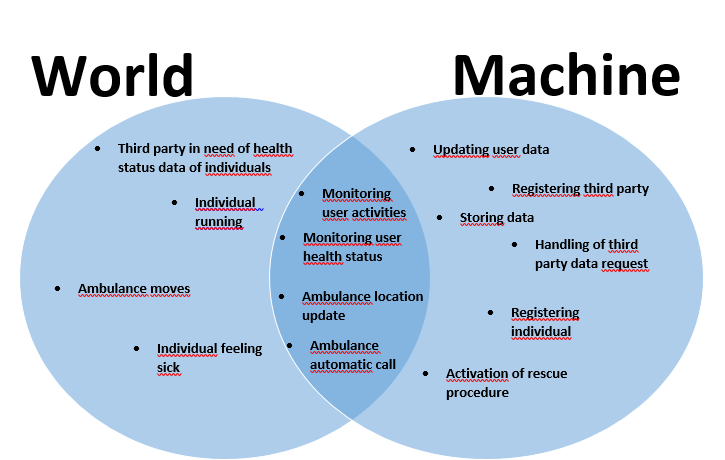
\includegraphics[scale=0.7]{img/phenomena.png}
\end{figure}


\subsection{Goals}

\begin{goal}
The users' eHealth data are correctly gathered from their device and uploaded to the system.
\end{goal}
\begin{goal}
Registered third-parties can access anonimized data.
\end{goal}
\begin{goal}
A registered third party can ask for permission to access an individual data.
\end{goal}
\begin{goal}
A registered third party can access the data of an individual who gave permission to it
\end{goal}
\begin{goal}
The system is able to start automatically a rescue procedure.
\end{goal}
\begin{goal}
The system is able to mantain the desired privacy level of each user (?).
\end{goal}
\begin{goal}
The system updates the third-party when new data of accepted requests is available
\end{goal}
\section{Definitions, Acronyms, Abbreviations}
\subsection{Definitions}
\begin{itemize}
\item \textbf{Rescue Procedure}: all the operations needed to save a person life. The operations include both the ones handled by computers and humans.
\item \textbf{eHealth Data}: all the data that can the related to the general health of the user, for example steps taken daily, hearth beat, blood pressure, activity level
\item \textbf{Health status}: level of health of a person, obtained analyzing various parameters like  hearthbeat rate, weight, hours of sleep.
\item \textbf{Critical Treshold}: value that, referred to an health parameter, must not be passed to guarantee user vital activities.
\end{itemize}




\subsection{Acronyms}

\begin{itemize}
\item \textbf{SSN}: Social Security Number
\item \textbf{TC}: Tax Code
\end{itemize}




\section{Revision History}
\section{Reference Documents}
\section{Document Structure}
\include{archdesign}
\include{graphicinterface}
\include{reqtrace}
\include{implinttest}
\chapter{Effort spent}\label{c:effort}
In the following tables the time spent for each section of the project is presented:

\renewcommand\arraystretch{1.5}
\begin{table}[ht]
\centering
\begin{tabular}{|l|l|}
\multicolumn{2}{c}{\textcolor{Blue}{\textbf{Stefano Pecchia}}} \\\hline
\multicolumn{1}{|c|}{\textbf{Section}} & \multicolumn{1}{|c|}{\textbf{Hours}} \\\hline
   Introduction, Component view, Deployment view, Requirements traceability & 3 
    \\ \hline
    Component interfaces, Selected architectural styles and patterns & 8
    \\ \hline
    Runtime view & 12
    \\ \hline 
    User interface design & see RASD
      \\ \hline 
    Implementation, integration and test plan & 4
	\\ \hline
	\end{tabular} \hspace{2.5em}
	\begin{tabular}{|l|l|}
\multicolumn{2}{c}{\textcolor{Blue}{\textbf{Edoardo Peretti}}} \\\hline
\multicolumn{1}{|c|}{\textbf{Task}} & \multicolumn{1}{|c|}{\textbf{Hours}} \\\hline

\end{tabular}
\end{table}
\chapter{References}

\begin{itemize}
\item Specification document "Mandatory Project Assignment AY 2018-2019.pdf"
\item ISO/IEC/IEEE 29148 - Standard on requirement engineering
\item WearOS by Google: https://wearos.google.com/\#hands-free-help
\item tool for building mockups: https://www.justinmind.com/
\item tool for uml diagrams: https://www.modelio.org/
\end{itemize}

\end{document}

